% Author: Theseas Maroulis
\documentclass[a4paper]{article}
\usepackage{xltxtra}
\usepackage[utf8]{inputenc}
\usepackage[greek]{babel}
\usepackage[a4paper, top=1.5cm, bottom=1.5cm, left=1.5cm,  right=1.5cm]{geometry}
\usepackage{amsmath, amssymb}
\usepackage{graphicx}
\usepackage{fancyhdr}
\usepackage{lastpage}
\usepackage{color}
\usepackage{tabularx}
\usepackage[usenames,table]{xcolor}
\usepackage{enumitem}
\usepackage{booktabs}
\usepackage{tikz}
\usepackage{multirow}
\usepackage[pdfauthor={Θησέας Μαρούλης (std101957@ac.eap.gr)}, pdftitle={Πλη11 Σημειώσεις}, colorlinks=true, linkcolor=blue]{hyperref}
\usepackage{listingsutf8}

\pagestyle{fancy}
\setmainfont[Mapping=tex-text]{DejaVu Sans}
\everymath{\displaystyle}
\renewcommand{\textdexiakeraia}{}

\begin{document}
% \chead{\large \color[HTML]{000090}\bfseries ΕΛΛΗΝΙΚΟ ΑΝΟΙΚΤΟ ΠΑΝΕΠΙΣΤΗΜΙΟ}
% \lfoot{\small{ΓΕ\_4 ΠΛΗ11-ΑΘΗΝΑ\_04 2015-2016}}
\title{Σημειώσεις πλη11}
\author{Θησέας Μαρούλης}
\date{\today}
\lhead{Σημειώσεις πλη11 - Θησέας Μαρούλης}
\lfoot{\small{Θησέας Μαρούλης}}
\cfoot{}
\rfoot{\small{\thepage/\pageref{LastPage}}}

\graphicspath{{./images/}}

\lstset{
	tabsize=4,
	language={C++},
	frame=single,
	keepspaces=true,
	%nunmbers=left,
	numbersep=5pt,
	breaklines=true,
	commentstyle=\color{gray},
	keywordstyle=\bfseries\color{blue}
}
\maketitle

\pagebreak
\tableofcontents

\section{Μοντέλα Κύκλου Ζωής Λογισμικού}

\subsection{Μοντέλο Καταρράκτη}

\begin{figure}[H]
	\centering
	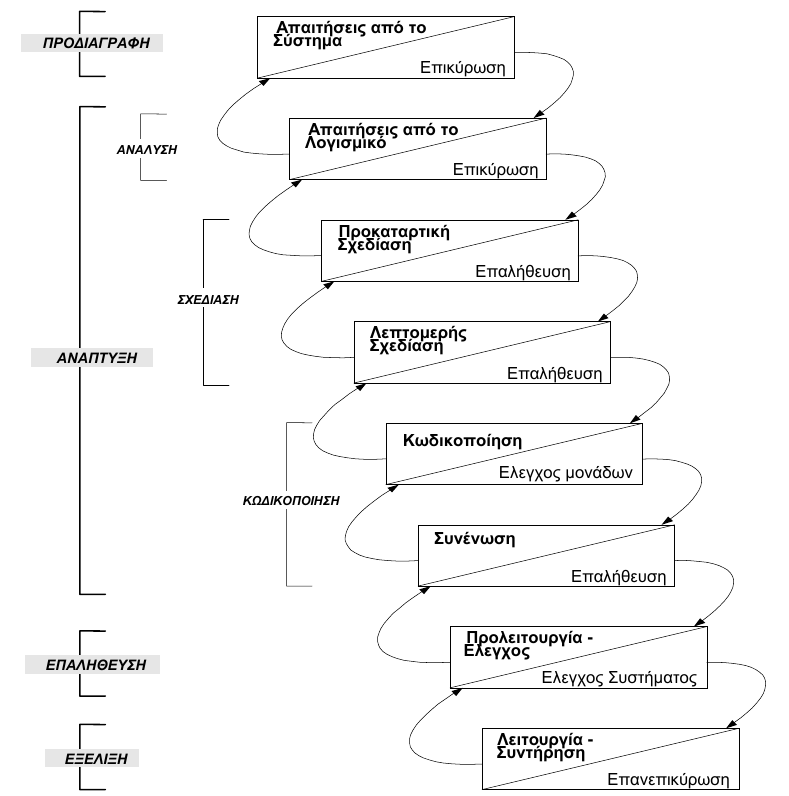
\includegraphics[width=0.6\textwidth]{waterfall.png}
	\caption{Waterfall model}
\end{figure}


\begin{itemize}
	\item	Καλό για μικρού ή μεσαίου μεγέθους εφαρμογές με απαιτήσεις
		εκ των προτέρων γνωστές.
	\item	Πρόβλημα αν αλλάξουν οι απαιτήσεις κατα την κατασκευή.
	\item	Διάδοση μεγάλη με τάσεις μείωσης.
\end{itemize}


\subsection{Μεντέλο Πρωτοτυποποίησης}

\begin{figure}[H]
	\centering
	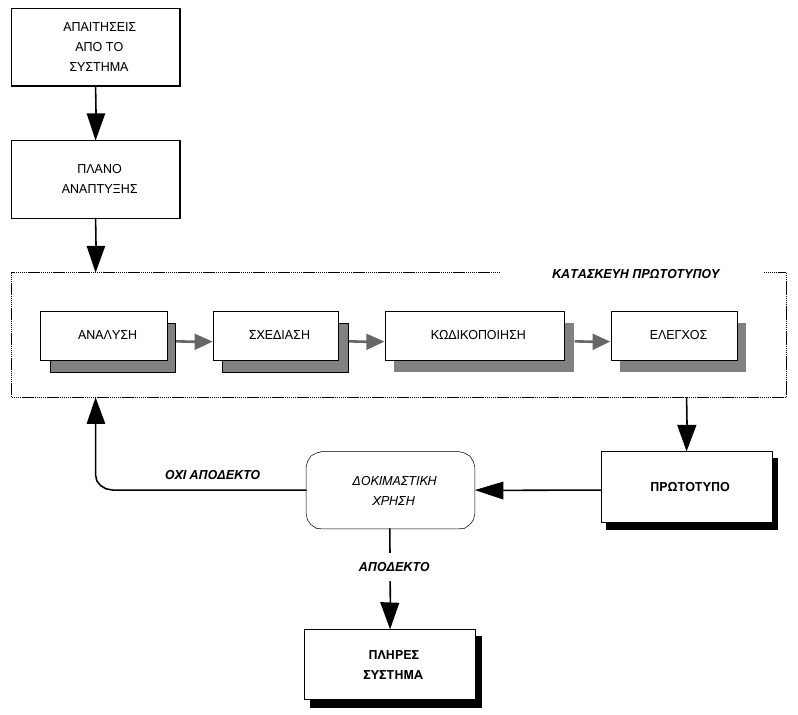
\includegraphics[width=0.6\textwidth]{prototyping.png}
	\caption{Prototyping Model}
\end{figure}

\begin{itemize}
	\item	επαναληπτικό μοντέλο που σε κάθε κύκλο κατασκευάζενται
		διαδοχικά πρότυπα με ολοένα περισσότερα χαρακτηριστικά αυτό να γίνει 
		αποδεκτό από τον πελάτη. Κάθε πρότυπο είναι ένα μικρό έργο λογισμικού 
		και μπορεί να χρησιμοποιεί άλλα μοντέλα.
	\item	ιδανικό για μικρές ή μεσαίες εφαρμογές που οι απαιτήσεις τους δεν είναι από την 
		αρχή γνωστές.
	\item	ιδιαίτερη σημασία αποκτά η διοίκηση του έργου.
	\item	διάδοση μικρή με τάσεις αύξησης
\end{itemize}

\subsection{Μοντέλο Λειτουργικής Επαύξησης}

\begin{figure}[H]
	\centering
	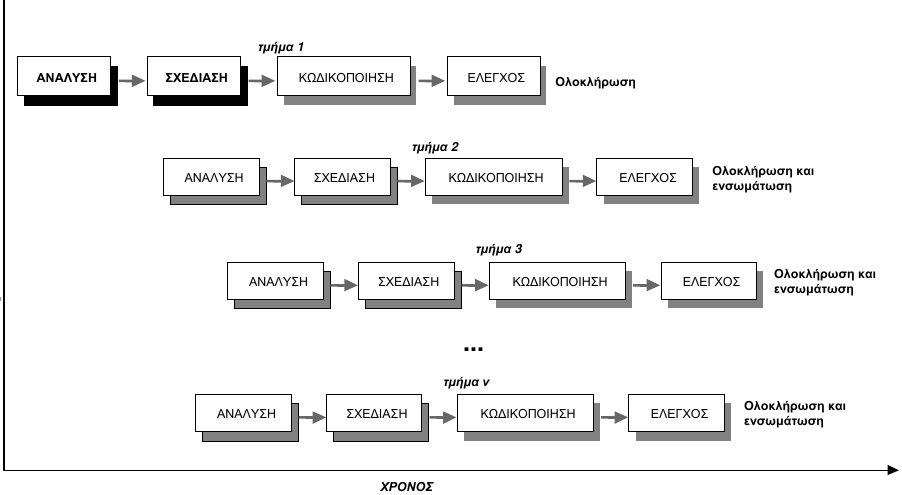
\includegraphics[width=0.6\textwidth]{incremental.png}
	\caption{Incremental Model}
\end{figure}

\begin{itemize}
	\item	Κατάτμηση του λογισμικού, εφαρμογή του μοντέλου του καταράκτη σε κάθε τμήμα και
		συνένωση του στο τέλος.
	\item	πλεονεκτήματα είναι η δυνατότητα παράλληλης ανάπτυξης, η οποία τελικά καταλάμβάνει
		μικρότερο χρόνο, καθώς και ο διαδοχικός εμπλουτισμός των λειτουργικών χαρακτηριστικών του.
	\item	μειονέκτημα: ιδιαίτερη βαρύτητα έχει η αρχική κατάτμηση του λογισμικού.
	\item	μειονέκτημα: Οι μεταβολές στις απαιτήσεις μπορεί να κλονίσουν την ανάπτυξη των υπόλοιπων τμημάτων.
	\item	Μεσαίος ως μεγάλο μέγεθος έργου με σαφείς απαιτήσεις από την αρχή.
	\item	διάδοση μικρή με τάση μείωσης.
\end{itemize}

\subsection{Σπειροειδές Μοντέλο}

\begin{figure}[H]
	\centering
	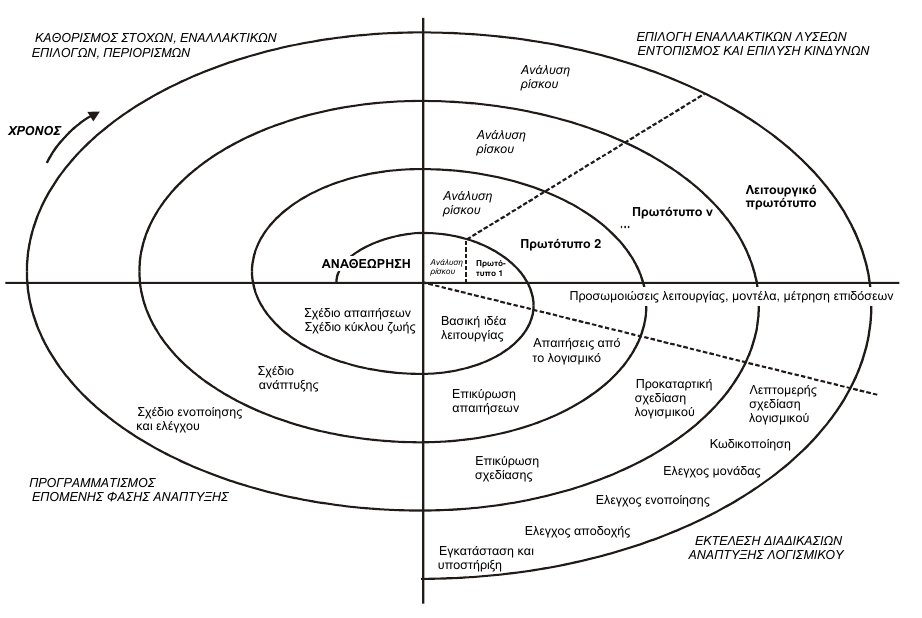
\includegraphics[width=0.6\textwidth]{spiral.png}
	\caption{Spiral Model}
\end{figure}

\begin{itemize}
	\item	Κύκλοι εργασιών με σταδιακή επέκταση των λειτουργικών χαρακτηριστικών της εφαρμογής.
	\item	Εκτίμηση ρίσκου σε κάθε κύκλο.
	\item	Μέγεθος εφαρμογής μεσαίο έως μεγάλο
	\item	Δεκτές οι μεταβολές στις απαιτήσεις
	\item	Αρκετή προσαρμοστικότητα στον κατασκευαστή.
	\item	Διάδοση μικρή με τάσεις μείωσης.
\end{itemize}

\subsection{Μοντέλο Πίδακα}

\begin{figure}[H]
	\centering
	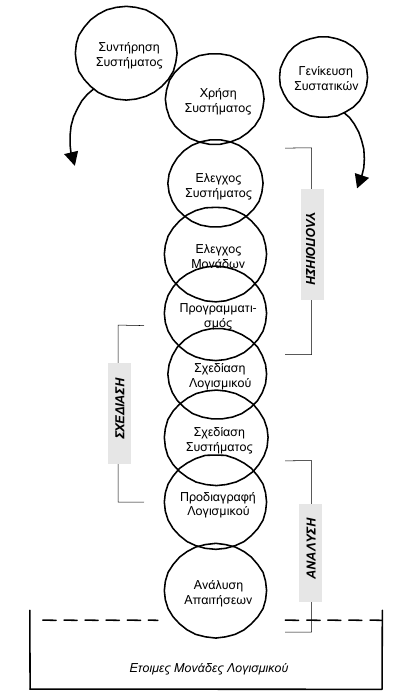
\includegraphics[width=0.6\textwidth]{object_oriented.png}
	\caption{Object Oriented Model}
\end{figure}

\begin{itemize}
	\item	Ανάπτυξη με αντικειμενοστρεφή φιλοσοφία και επαναχρησιμοποίηση έτοιμων συστατικών.
	\item	Κατάλληλο για οποιοδήποτε μέγεθος έργου.
	\item	Δεκτές οι μεταβολές στις απαιτήσεις.
	\item	Αρκετή προσαρμοστικότητα στον κατασκευαστή.
	\item	Διάδοση μικρή.
\end{itemize}

\subsection{Γενικό Μοντελό}

\begin{figure}[H]
	\centering
	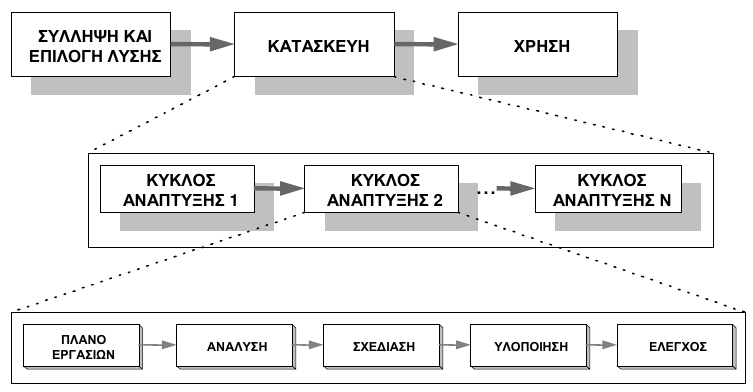
\includegraphics[width=0.6\textwidth]{general.png}
	\caption{General Model}
\end{figure}

\begin{itemize}
	\item	Ανάπτυξη σε κύκλους σύμφωνα με τα χαρακτηριστικά και τις δυνατότητες του κατασκευαστή.
	\item	Γενικευμένη μορφή των προηγούμενων μοντέλων κύκλου ζωής.
	\item	Δεκτές οι μεταβολές στις απαιτήσεις.
	\item	Κατάλληλο για οποιοδήποτε μέγεθος έργου.
	\item	Μεγάλη προσαρμοστικότητα στον κατασκευαστή.
	\item	Διάδοση μικρή με ισχυρές τάσεις αύξησης.
\end{itemize}


\section{Απαιτήσεις από το Λογισμικό}

\begin{itemize}
	\item	Λειτουργικές απαιτήσεις
	\item	Μη λειτουργικές απαιτήσεις
		\begin{itemize}
			\item	Απαιτήσεις χρήσης
			\item	Απαιτήσεις αξιοπιστίας
			\item	Απαιτήσεις επιδόσεων
			\item	Απαιτήσεις υποστήριξης
			\item	Απαιτήσεις σχεδίασης
			\item	Απαιτήσεις υλοποίησης
			\item	Απαιτήσεις επικοινωνίας με άλλα συστήματα
			\item	Απαιτήσεις βάσης δεδομένων
			\item	Φυσικές απαιτήσεις
		\end{itemize}
\end{itemize}

\pagebreak
\section{Διάγραμμα Ροής Δεδομένων}

\paragraph{Πηγή ή Αποδέκτης Δεδομένων}
Τα δεδομένα πρέπει πάντοτε να προέρχονται από κάπου και πρέπει να αποστέλλονται σε κάποιον.

\paragraph{Μετασχηματισμός Δεδομένων (αλλάζει την είσοδο σε έξοδο)}
Τα δεδομένα πρέπει πάντοτε να υπόκεινται σε επεξεργασία με
κάποιο τρόπο για να επιτευχθεί η λειτουργία του συστήματος.

\paragraph{Αποθήκη Δεδομένων}
Ο αριθμός των δεδομένων που γράφονται και διαβάζονται πρέπει να είναι ίδιος
στο συνολικό ΔΡΔ.

\begin{itemize}
	\item	Οι ροές εισόδου/εξόδου πρέπει προσεκτικά να καταγράφονται.
	\item	Στο επίπεδο 0 πάντοτε φαίνονται οι εξωτερικές οντότητες (πηγές / αποδέκτες).
	\item	Δώστε ετικέτα σε καθετί.
	\item	Οι εξωτερικές οντότητες μπορεί να επαναλαμβάνονται στο ίδιο διάγραμμα.
	\item	Οι εξωτερικές οντότητες  πρέπει να επαναλαμβάνονται σε όλα τα επίπεδα του ΔΡΔ,
		τουλάχιστον από μία φορά λόγω συνέπειας μεταξύ επιπέδων.
	\item	Κάθε φορά αναλύουμε ένα κύκλο (λειτουργία).
	\item	Η ανάλυση συνεχίζεται μέχρι κάθε κύκλος να αναπαριστά μια απλή και μοναδική λειτουργία 
		που συνδέεται με μια μόνο μονάδα προγράμματος.
	\item	Κάθε ροή δεδομένων (βέλος) μπορεί να αναλύεται στο επόμενο επίπεδο 
		(κάθε ροή δεδομένων καταγράφεται στο λεξικό δεδομένων).
	\item	Δεν περιγράφουμε διαδικαστική λογική (αλγόριθμο).
\end{itemize}

\begin{tabularx}{0.9\textwidth}{|X|X|X|X|}
	\hline
	{} & {Πηγή ή Αποδέκτης} & {Μετασχηματισμός} & {Αποθήκη Δεδομένων} \\
	\hline
	{Πηγή ή Αποδέκτης} & {X} & {\checkmark} & {X} \\
	\hline
	{Μετασχηματισμός} & {\checkmark} & {\checkmark} & {\checkmark} \\
	\hline
	{Αποθήκη Δεδομένων} & {X} & {\checkmark} & {X} \\
	\hline
\end{tabularx}

\begin{figure}[H]
	\centering
	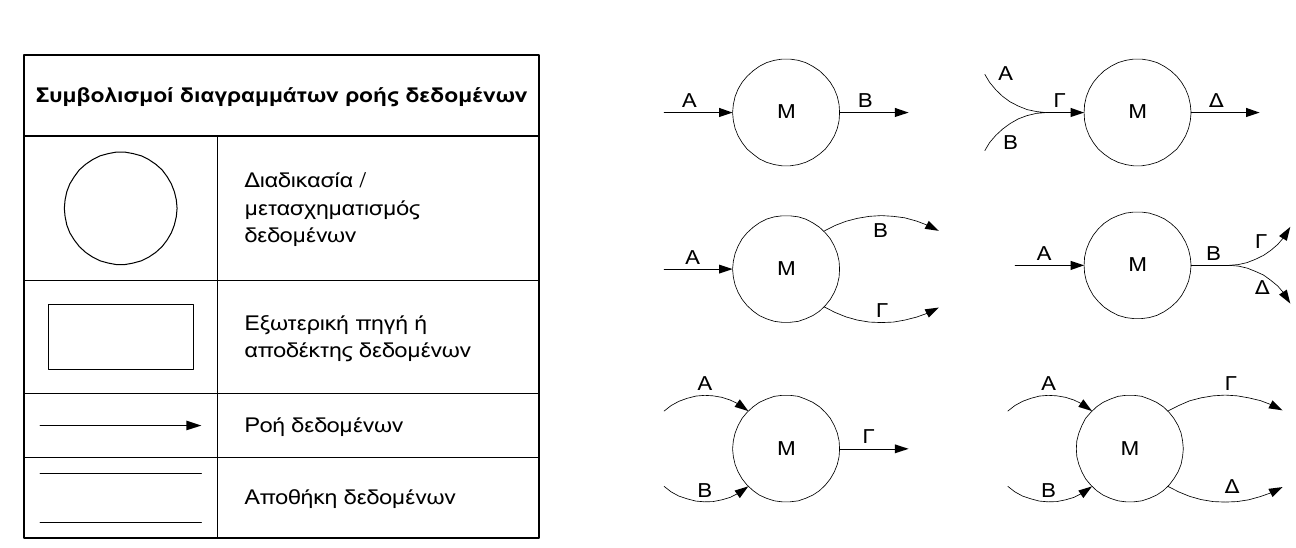
\includegraphics[width=0.9\textwidth]{drd.png}
	\caption{Συμβολισμοί \& Συμβάσεις ΔΡΔ}
\end{figure}


\section{Διάγραμμα Μετάβασης Καταστάσεων}

\begin{figure}[H]
	\centering
	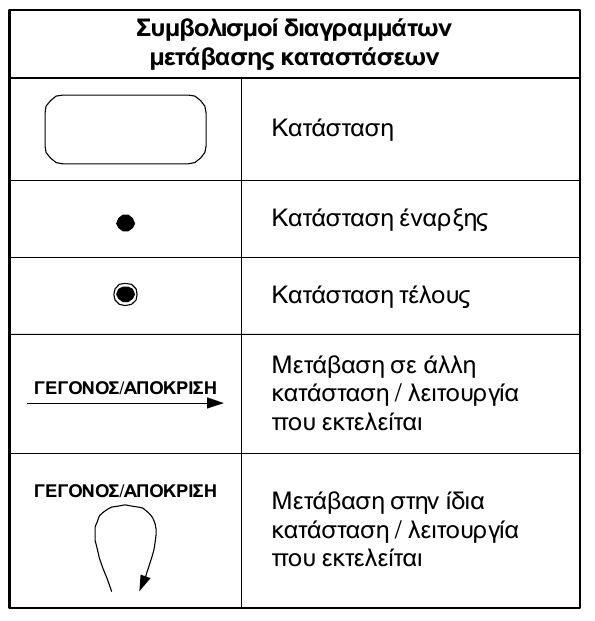
\includegraphics[width=0.5\textwidth]{dmk.png}
	\caption{Συμβολισμοί ΔΜΚ}
\end{figure}

\begin{enumerate}
	\item	Αναγνώριση της οντότητας
	\item	Αναζήτηση γεγονότων/αποκρίσεων
	\item	Αναζήτηση καταστάσεων – Αρίθμησή τους
	\item	Διασύνδεση καταστάσεων - γεγονότων
\end{enumerate}

\section{Λεξικό Δεδομένων}

Ένας πίνακας (ή μια Β.Δ.) που για κάθε στοιχείο δεδομένων περιέχει τουλάχιστον…

\begin{itemize}
	\item	Ονομασία: Το κύριο αναγνωριστικό της οντότητας, πεδίου ή ροής δεδομένων.
	\item	Βοηθητικές ονομασίες: Ονομασίες που χρησιμοποιούνται ισοδύναμα.
	\item	Πού χρησιμοποιείται: Αναφορά στους μετασχηματισμούς, οντότητες κλπ 
		οι οποίοι χρησιμοποιούν το εν λόγω στοιχείο.
	\item	Πώς χρησιμοποιείται: Αναφορά στον τρόπο με τον οποίο χρησιμοποιείται το εν λόγω στοιχείο
		(ως στοιχείο εισόδου, ως αποτέλεσμα, πεδίο, κ.ά.)
	\item	Τι περιέχει: Περιγραφή του είδους και της μορφής της πληροφορίας που αποθηκεύεται σε αυτό.
	\item	Όρια τιμών: Καθορισμός των επιτρεπτών τιμών που μπορεί να πάρει (αν απαιτείται).
	\item	Αρχική τιμή: Καθορισμός της αρχικής τιμής του στοιχείου (αν απαιτείται).
	\item	Λοιπά στοιχεία / συμπληρωματική πληροφορίας: Υπόλοιπες χρήσιμες πληροφορίες.
\end{itemize}


\section{SQL}

\subsection{Select}

\lstset{language=SQL}

\begin{lstlisting}[caption=select example]
select column1, column2, ... from table1 where ...; 
\end{lstlisting}

\begin{lstlisting}[caption=inner join example]
select column1, ... from table1 inner join table2 on table1.column_name=table2.column_name;
\end{lstlisting}

\begin{lstlisting}[caption=left join example]
select column1, ... from table1 left join table2 on table1.column_name=table2.column_name;
\end{lstlisting}

\begin{lstlisting}[caption=right join example]
select column1, ... from table1 right join table2 on table1.column_name=table2.column_name;
\end{lstlisting}

\begin{lstlisting}[caption=full join example]
select column1, ... from table1 full join table2 on table1.column_name=table2.column_name;
\end{lstlisting}

\begin{lstlisting}[caption=union example]
(select column(s) from table1) union 
(select column(s) from table2);
\end{lstlisting}

\begin{lstlisting}[caption=any example]
select columns from table1 where column1 = any 
(select column1 from table2);
\end{lstlisting}

\begin{lstlisting}[caption=all example]
select name from student where birth_date < all 
(select date from professor);
\end{lstlisting}

\begin{lstlisting}[caption=like example]
select * from table1 where column_name like pattern;
\end{lstlisting}

\begin{lstlisting}[caption=distinct example]
select distinct table1.column1, table2.column2, ... from table1, table2 where table1.column1=table2.column1;
\end{lstlisting}

\textbf{Προσοχή:} Oι στήλες που θα χρησιμοποιηθούν στα groub by, order by, having πρέπει να υπάρχουν στην επιλογή.

Η σειρά των εντολών είναι: select; from; where, group by, having, order by

\begin{lstlisting}[caption=order by example]
select column_name(s) from table1 order by column_name [asc|desc];
\end{lstlisting}

\begin{lstlisting}[caption=group by example]
select column_name(s) from table1 where column_name operator value group by column_name;
\end{lstlisting}

\begin{lstlisting}[caption=having example]
select column1, count(column1) from table1 group by column1 having count(column1)=1;
\end{lstlisting}

\subsection{Operators}

\begin{lstlisting}[caption=operators list]
=
<=
>=
>
<
<>
between <value> and <value>
like "%pattern%"
in (<set>)
is null
is not null
is not distinct from
as
\end{lstlisting}

\subsection{Εντολές Συνόλων}

\begin{lstlisting}[caption=set commands]
distinct
in
all
any
exists
not exists
unique
union
intersect
contains
except /* diafora 2 sunolwn */
\end{lstlisting}

\subsection{Create, Alter, Drop}

\begin{lstlisting}[caption=create database]
create database <name>;
\end{lstlisting}

\begin{lstlisting}[caption=create table]
create table <name> (id int not null, foreign_id int, ...,
primary key (id), foreign key (foreign_id) references table(foreign_id));
\end{lstlisting}

\begin{lstlisting}[caption=create view]
create view <name>
as select <columns> from <table>
where <condition>;
\end{lstlisting}

\begin{lstlisting}[caption=alter table]
alter table <name> add <column> <definition>;
\end{lstlisting}

\begin{lstlisting}[caption=drop]
drop database <name>;
drop table <name>;
drop view <name>;
\end{lstlisting}



\section{Λειτουργικά Συστήματα}

\lstset{language=C++}

\subsection{Παράλληλες διεργασίες}

\subsubsection{Γράφος προτεραιότητας – εντολές παραλληλισμού}

\begin{figure}[H]
	\centering
	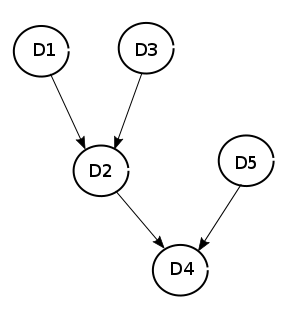
\includegraphics[width=0.4\textwidth]{grafos.png}
	\caption{Παράδειγμα Γράφου προτεραιότητας}
\end{figure}

\begin{lstlisting}[caption={Εντολές παραλληλισμού του παραπάνω παραδείγματος}]
cobegin
	begin
		cobegin
		D1;
		D3;
		coend;
		D2;
	end;
	D5;
coend;
D4;
\end{lstlisting}

\subsubsection{Συγχρονισμός} 


\paragraph{Κρίσιμες περιοχές - Αμοιβαίος αποκλεισμός}

\begin{itemize}
	\item 	Κρίσιμη περιοχή: Η περιοχή που περιέχει προσπελάσεις σε
		διαμοιραζόμενες περιοχές μνήμης ή αρχεία
	\item	Επιθυμητός ο αμοιβαίος αποκλεισμός: αποκλεισμός μιας
		διεργασίας από κάποια ενέργεια που ταυτόχρονα επιτελεί
		κάποια άλλη διεργασία
	\item	Λύση: Συγχρονισμός που προϋποθέτει τις ακόλουθες
		συνθήκες:
		\begin{enumerate}
			\item	Δυο διεργασίες δεν βρίσκονται ποτέ ταυτόχρονα στα κρίσιμα τμήματά
				τους (αμοιβαίος αποκλεισμός).
			\item	Δεν επιτρέπονται υποθέσεις σε ό,τι αφορά την ταχύτητα ή το πλήθος
				των επεξεργαστών.
			\item	Διεργασία που δεν βρίσκεται σε κρίσιμο τμήμα δεν επιτρέπεται να
				αναστείλει άλλες διεργασίες (progress).
			\item	Δεν επιτρέπεται η επ’ αόριστον αναμονή μιας διεργασίας για να
				εισέλθει στο κρίσιμο τμήμα της (bounded waiting).
		\end{enumerate}
\end{itemize}

\paragraph{Κρίσιμη περιοχή - Υλοποίηση}

\indent Πως μπορεί να υλοποιηθεί μια κρίσιμη περιοχή;
με «έξυπνες» λύσεις που βασίζονται στο λογισμικό
με τη χρήση «εργαλείων» που προσφέρουν τα ΛΣ
(αλλά και κάποιες – παλαιότερες - υψηλές γλώσσες
προγραμματισμού) όπως είναι οι σημαφόροι και οι
κρίσιμες περιοχές / κρίσιμες περιοχές υπό συνθήκη
με τη χρήση των δυνατοτήτων του hardware (π.χ. η
συνάρτηση TestAndSet)

\subsubsection{Mutex - Peterson}

Οι interested0,1 εκφράζουν πρόθεση να μπουν στην κρίσιμη περιοχή, 
ενώ η turn δηλώνει ποιος έχει σειρά να μπει.


\begin{lstlisting}[caption=Init Values]
turn = 0;
interested0 = false;
interested1 = false;
\end{lstlisting}

\begin{lstlisting}[caption=Process P0]
while(true){
	interested0 = true;
	turn = 0;
	while(interested1==true && turn == 0){}
	critical_section();
	interested0 = false;
	non_critical_section();
}
\end{lstlisting}

\begin{lstlisting}[caption=Process P1]
while(true){
	interested1 = true;
	turn = 1;
	while(interested0==true && turn == 1){}
	critical_section():
	interested1 = false;
	non_critical_section();
}
\end{lstlisting}

\subsubsection{Mutex - Dekker}

Αν και οι δύο διεργασίες θέλουν να
εισέλθουν στην κρίσιμη περιοχή, θα
θέσουν τις αντίστοιχες μεταβλητές true.
Η μεταβλητή turn θα λειτουργήσει τότε ως
διαιτητής για να αποτρέψει τη λιμοκτονία
(starvation) δηλαδή το να μη μπορεί καμία
διεργασία να μπει στην κρίσιμη περιοχή.

\begin{lstlisting}[caption=Init values]
turn = 1;
interested0 = false;
interested1 = false;
\end{lstlisting}

\begin{lstlisting}[caption=Process P0]
while(true){
	interested0 = true;
	while(interested1==true){
		if(turn==1){
			interested0 = false;
			while(turn==1){}
			interested0 = true;
		}
	}
	critical_section():
	turn = 1;
	interested0 = false;
	non_critical_section;
}
\end{lstlisting}

\begin{lstlisting}[caption=Process P1]
while(true){
	interested1 = true;
	while(interested0==true){
		if(turn==0){
			interested1 = false;
			while(turn==0){}
			interested1 = true;
		}
	}
	critical_section();
	turn = 0;
	interested1 = false;
	non_critical_section();
}
\end{lstlisting}

\subsection{Σημαφόροι}

\begin{lstlisting}[caption=wait or P or down function implementaion]
void signal(int *s){
	while(*s<=0) {}
	*s = *s - 1;
}
\end{lstlisting}

\begin{lstlisting}[caption=signal or V or up function implementaiton]
void wait(int *s){
	*s = *s + 1;
}
\end{lstlisting}

\begin{lstlisting}[caption=General semaphore implementation]
void wait(semaphore *u){
	u->count--;
	if(u->count < 0){
		*u.queue.push(this_process);
		this_process.block();
	}
}

void signal(semaphore *u){
	u->count++
	if(u->count<=0){
		*u.queue.pop();
		*u.ready_queue.push(this_process);
	}
}
\end{lstlisting}

Κάθε σημαφόρος διαθέτει μια ουρά στην οποία συνδέονται οι διεργασίες που
έχουν ανασταλεί λόγω της εκτέλεσης ενός wait (συχνά αναφερόμαστε σε αυτές
ως «μπλοκαρισμένες διεργασίες»).

\subsubsection{Ορισμός σημαφόρου}

\begin{itemize}
	\item	Υψηλότερου επιπέδου δομή για να πετύχουμε αμοιβαίο αποκλεισμό
	\item	Μέσω δύο πράξεων
		\begin{itemize}
			\item	Wait (S) ή P(S) ή Down(S)
			\item	Signal (S) ή V(S) ή Up(S)
		\end{itemize}
	\item	Μια εντολή σημαφόρου (wait ή signal) με ευθύνη
		του ΛΣ εκτελείται ατομικά, δηλ. αν μια διεργασία
		αρχίσει να εκτελεί π.χ. ένα wait σε ένα σημαφόρο,
		δεν επιτρέπεται να διακοπεί και η εκτέλεσή του
		wait αντιμετωπίζεται ως ένα αδιαίρετο βήμα.
\end{itemize}

\subsubsection{Είδη σημαφόρων}

\begin{itemize}
	\item	Βinary
		\begin{itemize}
			\item	Παίρνει τιμές 0 και 1
			\item	Προστατεύει την προσπέλαση των κρίσιμων περιοχών
			\item	mutex
		\end{itemize}
	\item	Γενική σημαφόρος
		\begin{itemize}
			\item	Μπορεί να παίρνει οποιαδήποτε θετική τιμή
		\end{itemize}
\end{itemize}

\textbf{Προσοχή:} Όλοι οι σημαφόροι πρέπει να είναι αρχικοποιημένοι!!!

\subsubsection{Προστασία κρίσιμων περιοχών}

Έστω δύο διεργασίες Α και Β που ενεργούν
πάνω στο υπόλοιπο Χ ενός λογαριασμού τράπεζας:

\begin{lstlisting}
semaphore mutex = 1; // mutex init value

void process_a(){
	wait (mutex);
	X = X + amount;
	signal (mutex);
}

void process_b(){
	wait (mutex);
	X = X - amount;
	signal (mutex);
}
\end{lstlisting}

\subsubsection{Συγχρονισμός διεργασιών}

Έστω δύο διεργασίες Α και Β. H A τυπώνει τη
λέξη ping και η Β τη λέξη pong:

\begin{lstlisting}
semaphore sem_a = 1;
semaphore sem_b = 0;

void process_a(){
	wait(sem_a);
	print("ping");
	signal(sem_b);
}

void process_b(){
	wait(sem_b);
	print("pong");
	signal(sem_a);
}
\end{lstlisting}

\subsubsection{Αναγνώστες και Συγγραφείς}

\begin{lstlisting}
semaphore rc_sem, write_sem = 1;
int readcount = 0;

void reader(){
	wait(rc_sem);
	readcount++;
	if(readcount = 1)
		wait(write_sem);
	signal(rc_sem);
	
	read(myfile, 'r');
	
	wait(rc_sem);
	readcount--;
	if(readcount = 0)
		signal(write_sem);
	signal(rc_sem);
}

void writer(){
	wait(write_sem);
	write(myfile, 'w');
	signal(write_sem);
}
\end{lstlisting}


\subsubsection{Χρονοδρομολόγηση διεργασιών}

\begin{itemize}
	\item	\textbf{Μη - Προεκχωρητικοί αλγόριθμοι:}
		Επιτρέπουν στις επιλεγμένες διεργασίες να κρατήσουν την
		ΚΜΕ μέχρι να ανασταλεί ή να τερματίσει.
	\item	\textbf{Προεκχωρητικοί αλγόριθμοι:}
		Η εκτέλεση της διεργασίας που κατέχει την ΚΜΕ
		διακόπτεται περιοδικά και ο χρονοδρομολογητής καλείται
		να αποφασίσει ποια θα είναι η επόμενη.
	\item	Μετρικές απόδοσης
		\begin{itemize}
			\item 	Χρόνος διεκπεραίωσης: $ \text{ΧΔ} = t_\text{περάτωσης εκτέλεσης} - t_\text{εισόδου στο σύστημα} $
			\item 	Χρόνος Αναμονής: $ \text{ΧΑ} = \text{ΧΔ} - t_\text{χρόνος εκτέλεσης εργασίας στην ΚΜΕ} $
			\item 	$ \text{Ρυθμός απόδοσης} = \frac{\text{Αρ. διεργ. που ολοκληρώνονται}}{t} $
			\item	$ \text{Χρόνος απόκρισης} = t_\text{έναρξης εξυπηρέτησης} – t_\text{υποβολής} $
		\end{itemize}
\end{itemize}

\paragraph{Αλγόριθμοι Χρονοδρομολόγησης}

\begin{itemize}
	\item	First Come First Served - FCFS
		\begin{itemize}
			\item	Δίκαιος Αλγόριθμος.
			\item	Παρουσιάζει πρόβλημα αν μια μεγάλη διεργασία μπει πριν από μια ή περισσότερες
				μικρές διεργασίες.
		\end{itemize}
	\item	Round Robin - RR (προεκχωρητική έκδοση FCFS)
		\begin{itemize}
			\item	Εξαιρετικά δίκαιος αλγόριθμός.
			\item	Δεν προκαλεί καθυστερήσεις στις μικρές διεργασίες, γεγονός που τον κάνει ιδανικό
				για συστήματα διαμοιρασμού χρόνου.
			\item	Αν το κβάντο χρόνου είναι µεγάλο, µπορεί να προκληθούν µεγάλοι χρόνοι
				απόκρισης σε µικρές αλληλεπιδραστικές διεργασίες.
			\item	Αν το κβάντο χρόνου είναι µικρό, εναλλαγές διεργασιών γίνονται πολύ συχνά, 
				γεγονός που µειώνει την αποδοτικότητα της ΚΜΕ.
		\end{itemize}
	\item	Shortest Job First - SJF
		\begin{itemize}
			\item	Όπως και ο αλγόριθμος προτεραιοτήτων μπορεί να προκαλέσει παρατεταμένη
				στέρηση για μεγάλες διεργασίες.
			\item	Πολύ δύσκολος στην υλοποίηση γιατί δεν γνωρίζουμε εκ των προτέρων πόσο
				χρόνο θα χρειαστεί η κάθε διεργασία.
		\end{itemize}
	\item 	Shortest Remaining Time First – SRTF (προεκχωρητική έκδοση SJF)
	\item	Priority
		\begin{itemize}
			\item	Δρομολόγηση διεργασιών βάση προτεραιοτήτων
			\item	Μπορεί να οδηγήσει σε παρατεταµένη στέρηση αν στο σύστηµα εισέρχονται διαρκώς
				διεργασίες µε µεγαλύτερες προτεραιότητες από εκείνη κάποιας άλλης διεργασίας.
		\end{itemize}
\end{itemize}

\subsection{Μνήμη}

\subsubsection{Σελίδοποίηση}

\begin{figure}[H]
	\centering
	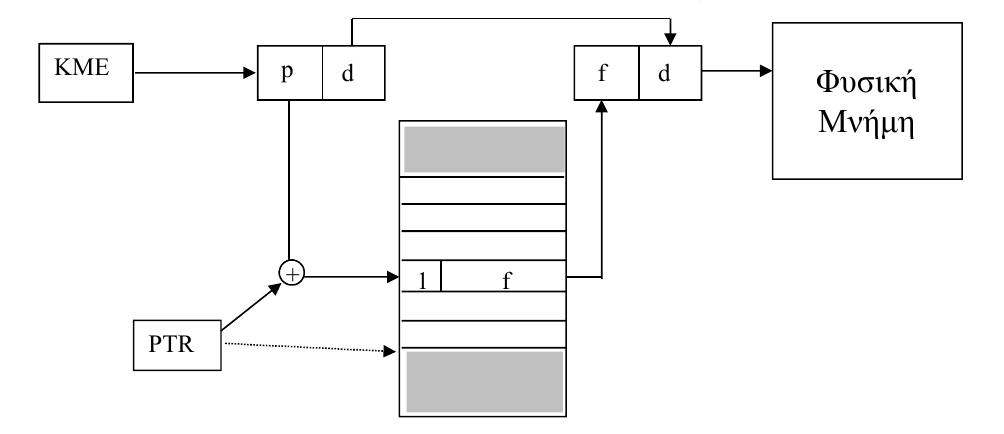
\includegraphics[width=0.5\textwidth]{paging.png}
	\caption{Paging}
\end{figure}

\begin{center}
\begin{tabularx}{0.5\textwidth}{|X|X|}
	\hline
	Όρος & Περιγραφή \\
	\hline
	p & Αριθμός σελίδας \\
	\hline
	f & Αριθμός Πλαισίου \\
	\hline
	d & Μετατόπιση (offset)\\
	\hline
	1 & Present bit (αν βρίσκεται η σελίδα στην μνήμη ή όχι) \\
	\hline
	ptr & {Page table register περιέχει τη διεύθυνση της φυσικής
	μνήμης όπου αρχίζει (έχει φορτωθεί) ο πίνακας σελίδων
	για την τρέχουσα διεργασία/πρόγραμμα } \\
	\hline
\end{tabularx}
\end{center}

\textbf{Προσοχή} Το + εδώ σημαίνει συνένωση όχι πρόσθεση!!! \\

\paragraph{Μορφή ιδεατής διεύθυνσης `U' (n bits):} Αριθμός Ιδεατής Σελίδας `p' (n-k bits) +
Μετατόπιση `d' (k bits) \\

\paragraph{Μετατροπή σε φυσική διεύθυνση Φ (σύνολο m bits):} Αριθμός φυσικής σελίδας `f' (m-k bits)  +
Μετατόπιση `d' (k bits)

\subsubsection{Μέσος Χρόνος Προσπέλασης Μνήμης}

Έστω ότι x (χρόνος προσπέλασης στους συσχετιστικούς καταχωρητές), y (χρόνος προσπέλασης της μνήμης),
p (ποσοστό επιτυχίας), p' ποσοστό αποτυχίας και $ 0 \le p, p' \le 1$, $ p + p' = 1$.

Για να υπολογίσουμε τον μέσο χρόνο προσπέλασης μνήμης (effective memory access time) κάνουμε:
$$ \text{Effective access time} = p \cdot (x+y) + p' \cdot (x+2y) $$

\subsubsection{Τμηματοποίηση}

\begin{figure}[H]
	\centering
	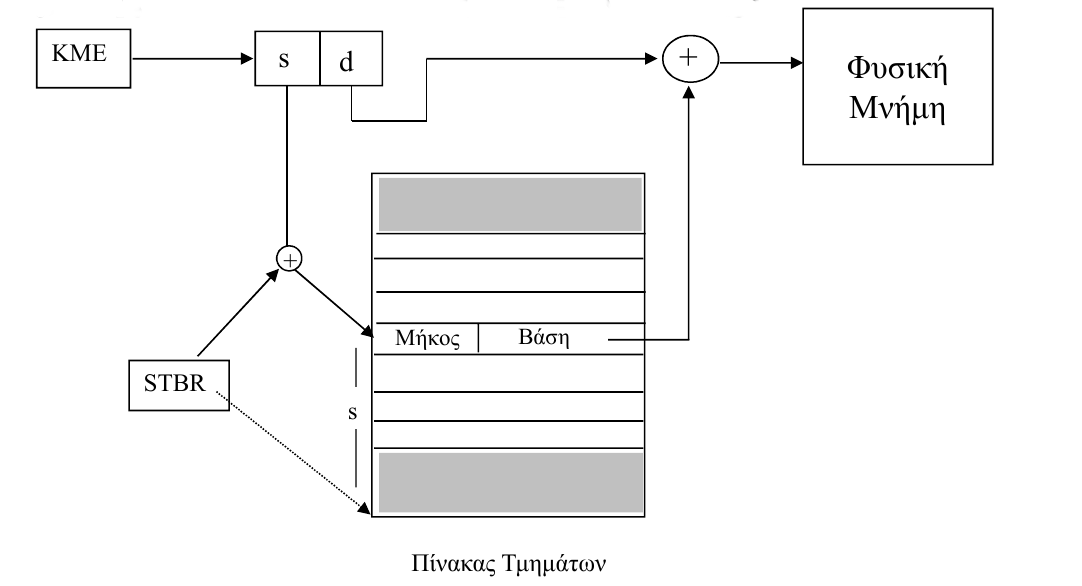
\includegraphics[width=0.5\textwidth]{segmentaion.png}
	\caption{segmentation}
\end{figure}

\begin{center}
\begin{tabularx}{0.5\textwidth}{|X|X|}
	\hline
	Όρος & Περιγραφή \\
	\hline
	s & Θέση στον πίνακα τμημάτων της διεργασίας \\
	\hline
	d & Μετατόπιση (offset). \textbf{Προσοχή} πρέπει να είναι μικρότερη από το μήκος. \\
	\hline
	STBR & {Segment Table Base Register: Σε ποια διεύθυνση
	της μνήμης αρχίζει ο πίνακας τμημάτων της διεργασίας μας} \\
	\hline
\end{tabularx}
\end{center}

\paragraph{Κάθε λογική διεύθυνση U (n bits) είναι στη μορφή:}
$$ \text{Αριθμός Λογικού Τμήματος }s (n-k~bits) + \text{ Μετατόπιση } d (k~bits) $$
$$ \text{Μέγιστος αριθμός τμημάτων: } 2^{n-k}\text{  Μέγιστο μέγεθος τμήματος: } 2^k $$
\paragraph{Μετατρέπεται σε μία Φυσική Διεύθυνση Φ στη μορφή:}
$$ \text{Διεύθυνση Βάσης Τμήματος } + \text{ Μετατόπιση } d (k~bits) $$

\subsubsection{Σελιδοποιημένη Τμηματοποίηση}

\paragraph{Η λογική διεύθυνση U (n bits) τώρα χωρίζεται σε 3 τμήματα.}
\begin{center}
\begin{tabularx}{0.95\textwidth}{|X|X|X|}
\hline
Αριθμός Τμήματος s(n-k bits) & \multicolumn{2}{|l|}{ + Μετατόπιση d (k bits)} \\
\hline
{} & Αρ. Σελίδας p & Μετατ. Σελίδας d' \\
\hline
\end{tabularx}
\end{center}

\paragraph{Και μετατρέπεται σε φυσική διεύθυνση Φ στη μορφή:}
\begin{center}
\begin{tabularx}{0.95\textwidth}{X X}
Αριθμός Φυσικής Σελίδας f(m-k' bits) & + Μετατόπιση d'(k' bits)
\end{tabularx}
\end{center}

\begin{figure}[H]
	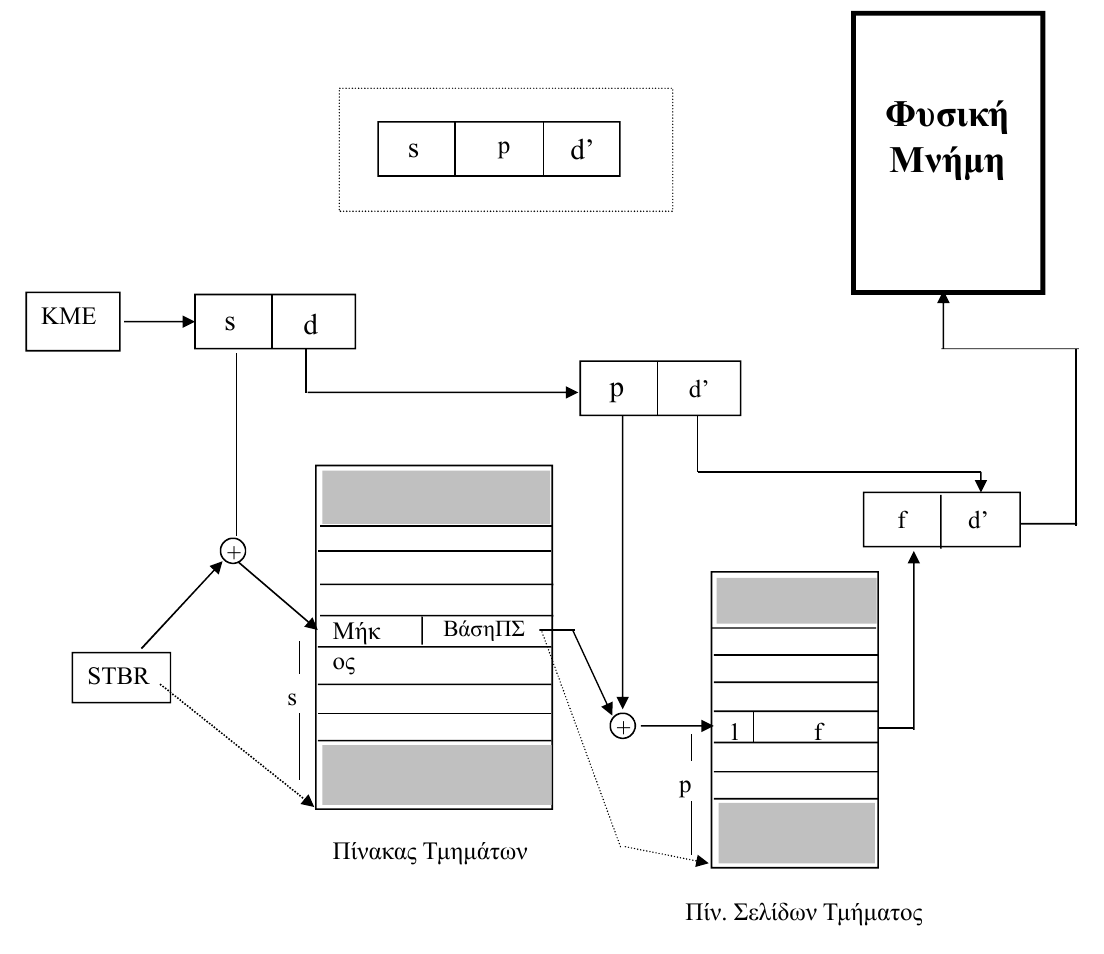
\includegraphics[width=0.75\textwidth]{paged_segmentation.png}
	\caption{Paged Segmentation (για τους όρους βλέπε τμηματοποίηση και σελιδοποίηση)}
\end{figure}

\subsubsection{Τμηματοποιημένη Σελιδοποίηση}

Οταν ο πίνακας σελίδων είναι πολύ μεγάλος...
\begin{itemize}
	\item	Μπορούμε να τον τμηματοποιήσουμε Segmented Paging = τμηματοποίηση του πίνακα σελίδων 
		σε περισσότερα (μεταβλητού μεγέθους) τμήματα.
	\item	Κάθε τμήμα του πίνακα σελίδων μπορούμε να το διαχειριστούμε
		ανεξάρτητα και είτε να βρίσκεται φορτωμένο στη μνήμη είτε όχι
		(ανάλογα με το αν χρησιμοποιείται συχνά από τη διεργασία).
	\item	Μεγάλα τμήματα στο τέλος του Πίνακα Σελίδων που είναι
		άχρηστα μπορούμε να τα διαχειριστούμε αποτελεσματικά χωρίς
		να καταλαμβάνουν χώρο στη μνήμη.
	\item	Καθώς έχουμε πολλαπλά μικρά τμήματα αντί ενός πολύ μεγάλου,
		είναι πιο εύκολη η διαδικασία εύρεσης και εκχώρησης
		ακολουθιακού χώρου μνήμης για κάθε ένα από αυτά
\end{itemize}


\paragraph{Η λογική διεύθυνση U (n bits) τώρα χωρίζεται σε 3 τμήματα.}

\begin{center}
\begin{tabularx}{0.95\textwidth}{|X|X|X|}
\hline
\multicolumn{2}{|l|}{Αριθμός Ιδεατής Σελίδας p(n bits)} & {Μετατόπιση d (k bits)} \\
\hline
Αρ. Τμήματος του Π.Σ. s & Μετατ. στο τμήμα p' & {} \\
\hline
\end{tabularx}
\end{center}

\paragraph{Και μετατρέπεται σε φυσική διεύθυνση Φ στη μορφή:}

\begin{center}
\begin{tabularx}{0.95\textwidth}{XX}
Αριθμός Φυσικής Σελίδας f(m-k' bits) & + Μετατόπιση d' (k' bits)
\end{tabularx}
\end{center}

Οπου m είναι τα bits της Τελικής Φυσικής Διεύθυνσης αν το
συνολικό μέγεθος αυτής θεωρηθεί 
$$ M = 2^m $$

\subsection{Αντικατάσταση σελίδων}
\begin{itemize}
	\item	Προστασία: χρήση ξεχωριστού πίνακα σελίδων για κάθε διεργασία.
	\item	Αλγόριθμοι αντικατάστασης:
		\begin{itemize}
			\item	First-In-First-Out (FIFO)
			\item	Least Recently Used (LRU)
			\item	Longest Residence in Memory (LRM)
			\item	Least Frequently Used (LFU)
		\end{itemize}
\end{itemize}

\subsubsection{FIFO}

Αντικατέστησε την παλαιότερη σελίδα (αυτή που έχει εισαχθεί πρώτη).
Προβλήματα:
\begin{itemize}
	\item	Μπορεί οι παλιές σελίδες να χρησιμοποιούνται συχνά.
	\item	Τα σφάλματα αναφοράς μπορεί να αυξηθούν 
		όσο αυξάνονται τα πλαίσια σελίδας!!! (Belady’s Anomaly)
\end{itemize}

\subsubsection{Αλγόριθμος $2^\text{ης}$ Ευκαιρίας}

\begin{itemize}
	\item	Βασίζεται στη στρατηγική FIFO: εξετάζει σελίδες αρχίζοντας
		από την πιο παλιά αλλά χρησιμοποιεί και bit αναφοράς.
	\item	1η αναφορά σε σελίδα και τοποθέτησή της σε πλαίσιο -> R = 1
	\item	Επιλέγει την πιο παλιά σελίδα και εξετάζει το R bit.
		\begin{itemize}
			\item	Αν R=0 τότε την αντικαθιστά και η νέα σελίδα έχει R = 1.
			\item	Αν R = 1 τότε
				\begin{itemize}
					\item	κάνει το bit R = 0
					\item	η σελίδα τοποθετείται στο τέλος της λίστας 
						(δηλ. "βαφτίζεται" σαν η πιο πρόσφατη σελίδα).
					\item	η αναζήτηση θύματος συνεχίζεται στην επόμενη πιο παλιά σελίδα.
				\end{itemize}
			\item	Αν R=1 για όλες τις σελίδες, τότε second-chance είναι στην ουσία FIFO, 
				γιατί κάνει τα R όλων των σελίδων 0 και μετά επίλέγει την παλιότερη όπως ο FIFO.
		\end{itemize}
\end{itemize}

\subsubsection{LRU}

\begin{itemize}
	\item	Αντικατέστησε τη σελίδα που δεν έχει χρησιμοποιηθεί για το μεγαλύτερο διάστημα.
	\item	Προβλήματα:
		\begin{itemize}
			\item	"Ακριβή" υλοποίηση: π.χ. Ανάγκη διατήρησης χρονικής πληροφορίας
				(time stamp) για κάθε σελίδα.
		\end{itemize}
\end{itemize}


\section{Διάφορες σημειώσεις}

\subsection{Πίνακας Μετατροπών}

\begin{center}
	\begin{tabular}{|c|c|c|c|}
	\hline
	Δεκαδικό & Δυαδικό & Δεκαεξαδικό & Οκταδικό \\
	\hline
	00 & 0000 & 0& 00 \\
	\hline
	01 & 0001 & 1& 01\\
	\hline
	02 & 0010 & 2& 02\\
	\hline
	03 & 0011 & 3& 03\\
	\hline
	04& 0100 & 4& 04\\
	\hline
	05& 0101 & 5& 05\\
	\hline
	06& 0110 & 6& 06\\
	\hline
	07& 0111 & 7& 07\\
	\hline
	08& 1000 & 8& 10\\
	\hline
	09& 1001 & 9& 11\\
	\hline
	10& 1010 & A& 12\\
	\hline
	11& 1011 & B& 13\\
	\hline
	12& 1100 & C& 14\\
	\hline
	13& 1101 & D& 15\\
	\hline
	14& 1110 & E& 16\\
	\hline
	15& 1111 & F& 17\\
	\hline
	\end{tabular}
\end{center}


\end{document}
